\documentclass[12pt,fleqn]{article}\usepackage{../../common}
\begin{document}
Materyel Mekaniği - 2

Kirişin Yatay Kesme Stresi

Birornek bukulmeye maruz olan bir kirisi dusunelim, 

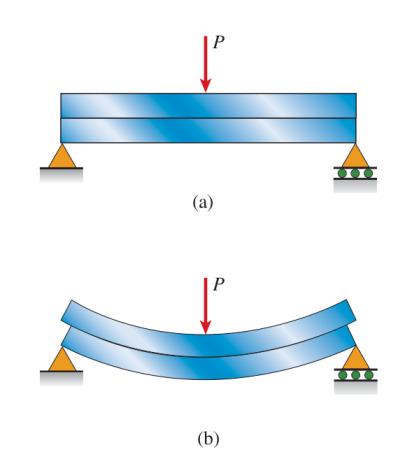
\includegraphics[width=15em]{phy_020_strs_02_02.jpg}

Kirisin bir bolumunu alttaki (a) resminde goruyoruz, simdi bu bolumdeki
$\ud x$ genisligindeki ufak bir parcaya odaklanalim,

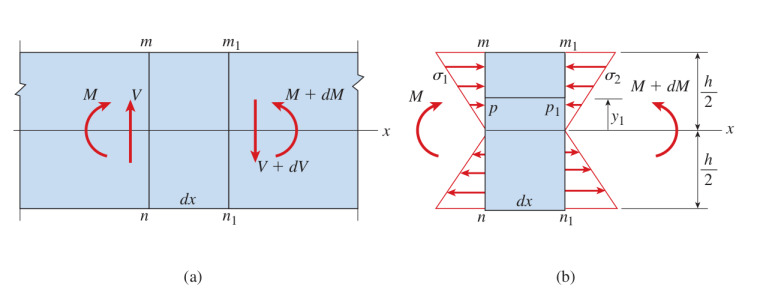
\includegraphics[width=30em]{phy_020_strs_02_01.jpg}

Bu ufak parçanın sol kısmına etki eden kesme kuvveti ve bükülme momenti
$V$ ve $M$. Eksene sağa gittikçe bu değerler değişik olabileceği için
parçanın sağında $V + \ud V$ ve $M + \ud M$ olacaktır. 

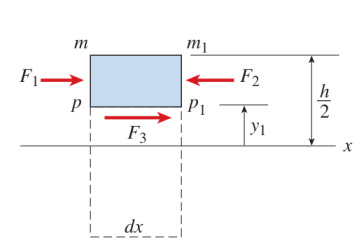
\includegraphics[width=15em]{phy_020_strs_02_04.jpg}

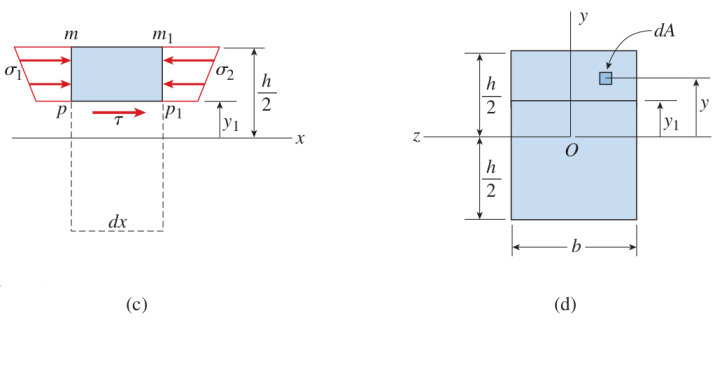
\includegraphics[width=30em]{phy_020_strs_02_03.jpg}

Bükülme normal stres (flexure) formülünden $\sigma = My / I$ olduğunu
biliyoruz. $\sigma_1$ için yerine koyalım,

$$
\sigma_1 \ud A = \frac{My}{I} \ud A
$$

Tum $F_1$ kuvveti icin tanimladigimiz alan uzerinden entegral alalim,

$$
F_1 = \int \sigma_1 \ud A = \int \frac{My}{I} \ud A
$$

$$
F_2 = \int \sigma_2 \ud A = \int \frac{(M + \ud M)y}{I} \ud A
$$

$$
F_3 = F_2 - F_1
$$

$$
F_3 = \int \frac{(M + \ud M)y}{I} \ud A -  \int \frac{My}{I} \ud A =
\int \frac{(\ud M)y}{I} \ud A
$$

$$
F_3 = \frac{\ud M}{I} \int y \ud A
$$


[devam edecek]

Kirişin Yatay Kesme Stresi - Alternatif Anlatım

Kesme stresi $\tau$'yu bulmak için yine kirişin ufak bir kısmına odaklanalım,

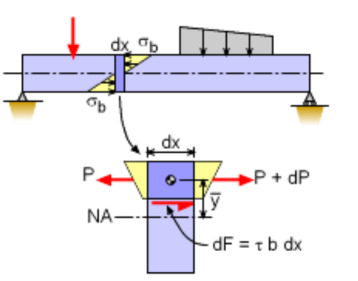
\includegraphics[width=15em]{phy_020_strs_01_05.jpg}

Tüm etki eden kuvvetlerin toplamı sıfır olmak zorundadır [3],

$$
-P + (P + \ud P) + \tau b \ud x = 0
$$

ki $b$ kesme stresinin uygulandığı noktadaki kiriş derinliğidir. 

$$
-\ud P/\ud x = \tau b
\mlabel{1}
$$

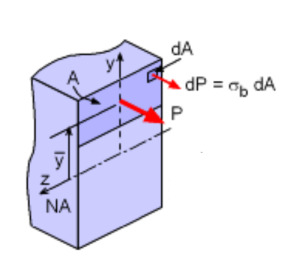
\includegraphics[width=15em]{phy_020_strs_00_01.jpg}

$P$'yi bulmak için $A$ bölgesindeki stresleri entegre ediyoruz,

$$
\int_A \ud P = \int_A \sigma_b \ud A
$$

Fakat daha önce bulduk ki $\sigma_b = -My / I$, yerine koyunca,

$$
P = \int_A - \frac{My}{I} \ud A
$$

$M$ ve $I$ sabittir, entegral dışına çıkartılabilir,

$$
P = - \frac{M}{I} \int_A y \ud A = - \frac{MQ}{I}
$$

ki görülen entegral bir alanın kütle merkezini bulmak için kullanılan standart
bir entegraldır, $Q = \int_A y \ud A$. Devam edelim üstte bulunan $P$'yi (1)'e
sokunca,

$$
- \frac{\ud}{\ud x} \left( - \frac{MQ}{I} \right) = \tau b
$$

$$
\frac{Q}{I} \frac{\ud M}{\ud x} = \tau b
$$

Şimdi hatırlarsak $\ud M/\ud x$ türevi yatay kesme / teğetsel yükü $V$'ye
eşittir. O zaman

$$
\frac{Q}{I} V = \tau b
$$

Nihai yatay kesme stres denklemi,

$$
\tau = \frac{V Q}{I b}
$$

Problemler

Altta kiriş odaklı bazı örnek problemleri çözeceğiz. Bir kirişe yük
uygulandığında dengenin muhafaza edilmesi için kiriş içinde kuvvetler oluşur.
Bu iç kuvvetler kirişin destek yapısına göre farklı şekillerde ortaya çıkabilir
[1].

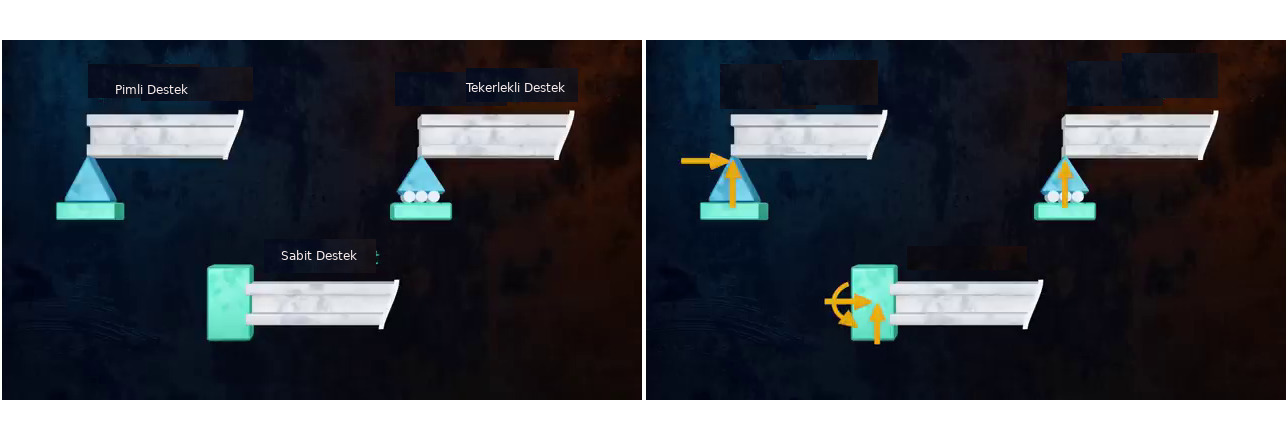
\includegraphics[width=25em]{phy_020_strs_01b_01.jpg}

Üstteki soldaki resimde mesela iki boyutta pimli destek dönüşe izin verir,
tekerlekli yatay sağ, sol hareketi ve dönüşü serbest bırakır. Sabit destekte hiç
harekete izin yoktur. Hangi harekete izin verilmediğine göre yük uygulanması
ardından üst sağdaki iç kuvvetler ortaya çıkacaktır, bunlar pimli durumda dikey
ve yatay kuvvetler, tekerlekli durumda dikey kuvvet, sabit durumda ise her üç
mümkün tepkilerdir, yani moment, dikey ve yatay.

Yükler noktasal ya da dağıtık şekilde uygulanabilir, altta noktasal kuvvet,
dağıtık kuvvet ve noktasal moment örneklerini görüyoruz.

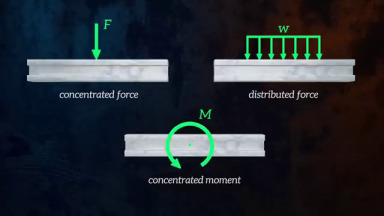
\includegraphics[width=20em]{phy_020_strs_01b_02.jpg}

Tipik olarak problemin beklediği kesim kuvveti ve bükülme momenti grafikleridir,
bu grafiklerde $x$ ekseni yatay olarak kirişin kendisi, $y$ ekseni ise o noktada
etki eden kesim ya da moment büyüklüğüdür.

Çözme yöntemi olarak iki yaklaşım mevcut, biri her kritik noktada kirişin
hissettiği içsel kuvvetler ve momentleri hesaplamak için o noktalarda denge
denklemlerini kullanmak, ki bu denklemlere (ve temel fiziğe göre) kirişe
uyguladığımız hayali bir kesitte etki eden tüm kuvvetler ve momentler birbirini
dengelemeli. Ardından bu kesit tüm kiriş boyunca kaydırılır ve gereken kuvvetler
aynı denge üzerinden hesaplanır. Eğer tüm yükler noktasal ise bu yaklaşım iyi
işler.

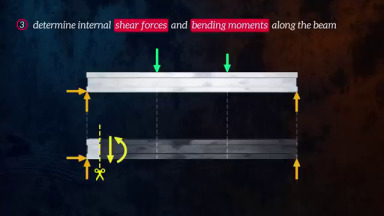
\includegraphics[width=20em]{phy_020_strs_01b_03.jpg}

Bir diğer yaklaşım Calculus kullanmak. Bu yaklaşım temelde sürekli bazda çözüm
verdiği için dağıtık yük durumunda daha kolay işler, kritik noktalara odaklanmak
yerine pür formulsel düşünebiliriz . Daha önce görmüştük ki kesim kuvvet
formülünün eğimi (türevi) o noktadaki uygulanan yükün negatifidir
$\ud V / \ud x = -w$, ve bükülme moment grafiğinin eğimi ise o noktadaki
kesim kuvvetine eşittir, $\ud M / \ud x = V$.

Problem 1














[devam edecek]

Kaynaklar 

[1] The Efficient Engineer, {\em Understanding Shear Force and Bending Moment Diagrams},
    \url{https://youtu.be/C-FEVzI8oe8}

[2] Gere, {\em Mechanics of Materials}

[3] Gramoll, {\em Mechanics},
    \url{http://www.ecourses.ou.edu/cgi-bin/ebook.cgi?topic=me}

\end{document}

